%%-------------------------------------------------------------------------------
\section{Introduction}
%%-------------------------------------------------------------------------------
Dataflow analysis is a fundamental technique in software enginering that tracks which variables can influence each other and how information flows through a program ~\cite{kildall1973unified, fosdick2011data}. For security applications, a type of dataflow analysis called taint tracking is typically used, which tracks dataflows between a specified set of sources and sinks in a program ~\cite{newsome2005dynamic}. Taint tracking has multiple applications in security, including detecting attacks at run time, guided fuzzing, discovering information leaks, and malware analysis ~\cite{clause2007dytan, schwartz2010all, ganesh2009taint, rawat2017vuzzer, arzt2014flowdroid, yan2012droidscope}. It can be performed either statically, by analyzing the source code or binary of a program, or dynamically, by instrumenting a program and tracking taint as it executes. However, static analysis cannot distinguish invalid program states that cannot be reached during execution, leading to high false positive rates ~\cite{jovanovic2006pixy}. Dynamic taint analysis avoids this problem by operating on concrete executions, but still suffers from two limitations: it uses overapproximations in its propogation rules that still lead to high false positive rates, and it only operates on individual inputs, providing no information about overall program behavior ~\cite{balzarotti2008saner}. 

The overappoximations in dynamic taint tracking come from two sources: numerical errors on single instructions, and compound errors involving multiple instructions. Numerical errors occur when instructions inputs may or may not effect the output depending on their values. For example, in the operation \tc{y = x1 - x2;} both \tc{x1} and \tc{x2}  clearly effect the output \tc{y}, leading to the propogation rule $taint(y) = taint(x1) \cup taint(x2)$, but if the operation happens on the same variable \tc{y = x - x} this propogation will be incorrect. Compound errors occur when taint is propogated over sequence of operations that are handled correctly individually but incorrect in aggregate. In the two operations \tc{a = x1 + x2; b = a - x1;}, a taint propogation will indicate $taint(b) = taint(x1) \cup taint(x2)$, when in fact the value of $x1$ has no effect on $b$, and $taint(b) = taint(x2)$. The combined effect of these errors is that entire sections of a program will be incorrectly tainted during execution, making dynamic taint tracking impractical for most real world applications. \gabe{should we mention underapproximations from memory etc here too? We could argue we can address it with sampling, but it isn't implemented yet...}


%\begin{figure}
  %\centering
  %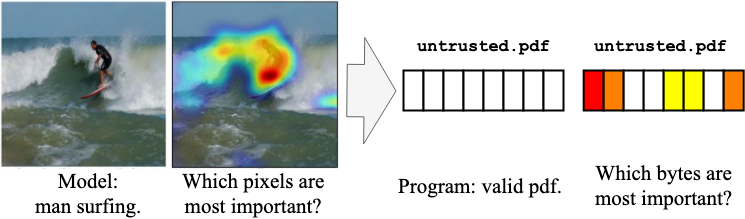
\includegraphics[width=\linewidth]{figs/sosp-nn_explain2}
  %\vspace{-15pt}
  %\caption{\label{fig:nn_analogy} Examples of gradient based explanations for machine learning model and program behavior ~\cite{selvaraju2017grad}.}
  %\vspace{-15pt}
%\end{figure}


To address these limitations, we draw inspiration from the fields of statistical modeling and optimization, in which gradients have long been used as a method for analyzing model behavior ~\cite{cook1986assessment}. Recently, gradients have been used for a variety of tasks that are analagous to dataflow analysis on programs, such as explaining model behavior, generating adversarial examples, and maximizing test coverage  ~\cite{baehrens2010explain, simonyan2013deep, shrikumar2017learning, goodfellow2014explaining, pei2017deepxplore}. In these applications, gradients serves as a measure of how inputs to a model determine its behavior, making it possible to explain that behavior or generate new inputs that alter the behavior. Dataflow in programs is similarly used to identify important inputs, discover vulnerabilities, and measure test coverage ~\cite{ganesh2009taint, rawat2017vuzzer, newsome2005dynamic, hutchins1994experiments}. 

%To address these limitations, we draw inspiration from the deep learning community, where accurately identifying which inputs explain why a model made a given decision is an active area of research. Conceptually, explaining model decisions is a dataflow problem, in which the input data that most strongly affects the model decision, and therefore flows to the output, should be identified. Many of these explanation methods rely on local gradient with regard to input, which is the slope of the model, or the measure of how change in the input changes the output for a given input ~\cite{baehrens2010explain, simonyan2013deep, shrikumar2017learning}. Intuitively, gradient serves as indication of how inputs effect outputs for differentiable models.



As a method for dataflow analysis, tracking gradients between variables within a program can address both limitations of taint tracking. In cases where taint would over approximate due to numerical or compound errors, such as operations like \tc{y = x - x;} the gradient $\tfrac{dy}{dx}$ is naturally $0$, so no overapproximation will occur. Moreover, gradient gives additional information by indicating how each of the source variables effect a given sink, which can be used to identify which sources are most significant or guide a search for vulnerabilities. Figure \ref{fig:taint_v_gradient} shows how these advantages can combine to cut out false positives and distinguish the most important inputs that can trigger a specific error in a program.


\begin{figure}
  \centering
  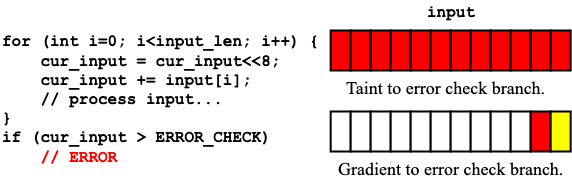
\includegraphics[width=\linewidth]{figs/sosp-grad_v_taint_ex}
  \vspace{-25pt}
  \caption{\label{fig:taint_v_gradient} Example of a program in which an iterated shift operation on the input will cause overtainting, while gradient will correctly identify which input bytes are most influential in triggering an error. \gabe{can change colors if this looks too much like a firetruck}}
  \vspace{-15pt}
\end{figure}

However, gradients cannot be computed over programs in the same way they are on continuous systems. In a continuous system, each operation is differentiable, so the gradients of individual operations can be composed via the chain rule to compute a gradient over the entire model ~\cite{Wengert:1964:SAD:355586.364791}. In contrast, programs contain many operations that are discrete and have nonsmooth behavior, such as bitwise operators and branches, which cannot be differentiated directly \gabe{should we just say nondifferentiable instead of nonsmooth? nonsmooth may be confusing.}. These nondifferentiable operations break the chain rule and prevent the gradient from being computed. Therefore, in order to evaluate gradients over programs, we use methods developed for nonsmooth optimization that relax the chain rule to apply to nondifferentiable functions. In particular, we use proximal gradients, a type of gradient approximation that is widely used to solve optimization problems with nondifferential objective functions ~\cite{parikh2014proximal}. 

Proximal gradients estimate the local gradient by finding a nearby minima of a function and drawing a line to it. They have two properties that make them well suited to working with nonsmooth operations in programs. First, they are robust to the discrete and nonsmooth behavior that makes program operations nondifferentiable, such that performing optimization with proximal gradients is proven to find a local minimum ~\cite{bertsekas2015convex}. Second, proximal gradients use a soft bound to limit the region in which they operate, making it possible to evaluate them without sampling all possible inputs to a function. 

To apply proximal gradients to nonsmooth operations in programs, we first derive bounds on the region which must be sampled to evaluate the proximal gradient. We base our analysis on the observation that operations in programs are Lipschitz continuous, meaning that their gradients are bounded. We then use these bounds on gradient to derive sampling bounds on proximal gradients for any function that is Lipschitz continuous. After defining the proximal gradient for individual operations, we show it can be applied to entire programs by modeling the program as a composition of functions and applying the relaxed chain rule. We then define methods for propogating Lipschitz bounds and proximal gradients over each type of nonsmooth operation in a program, creating a theoretically grounded framework for gradient analysis of programs.

We implement proximal gradient analysis as an LLVM pass that instruments programs during compilation to compute proximal gradients for each operation. To evaluate gradient analysis, we compare it to DataFlowSanitizer, LLVM's implementation of taint tracking. We measure performance on 7 widely used file parsing programs, and show that our implementation of gradient analysis achieves up to 42\% better precision while introducing lower average overhead than DataFlowSanitizer. Next, we apply it to guided fuzzing, and show that a gradient guided fuzzer achieves higher coverage faster than a taint guided fuzzer. Finally, we show that gradient analysis can also detect X out of X known CVEs that are detected by taint tracking.

In addition to performing comparative evaluations, we demonstrate that gradient analysis is an effective tool for finding new bugs. By instrumenting programs to track gradients to potentially vulnerable function calls and arithmetic operations and using the recorded gradients to craft new inputs, we found a total of X new bugs on our test programs, including integer overflow errors, buffer overflow errors, memory allocation errors, and memory leaks.

The rest of this paper is organized as follows: First, section 2 provides background on the methods that we use proximal gradient analysis. Next, in section 3, we provide a working example of evaluating a proximal gradient. Section 4 then shows how these methods can be combined to evaluate gradients over programs. Section 5 gives an overview of our implementation, and section 6 provides the details of our evaluations and results. Finally, we address related work in section 7, and present conclusions and future directions for further work in section 8.

Our main contributions are:

\vspace{-1pt}
\begin{enumerate}
\item We introduce a novel form program analysis, Proximal Gradient Analysis, that is theoretically grounded in Nonsmooth Optimization methods and able to evaluate useful gradients over a program.
\item We implement a framework for tracking gradients using Proximal Gradient Analysis as an LLVM pass, and provide open source code for use by the community.
\item We evaluate Proximal Gradient Analysis in comparison to taint tracking on dataflow analysis, guided fuzzing, and CVE detection, and show that it achieves up to 42\% better precision, X\% better coverage, and can detect X out of X CVEs while introducing lower average overhead than taint tracking.
\item We demonstrate that Proximal Gradient Analysis is an effective technique for finding bugs, and find X bugs across 7 programs, including memory corruption bugs, memory allocation bugs, and undefined behavior bugs.
\end{enumerate}
\vspace{-5pt}




%On operations where it is not possible to evaluate the gradient directly, we instead evaluate the Proximal Gradient, which estimates the gradient by sampling the function in a local region. \gabe{explain how prox grad addresses nonsmooth issue}






%\gabe{here be the old intro.}

%Discovery of new security vulnerabilities is a fundamentally difficult problem because the space of possible inputs to a program is exponentially large. However, the inputs that significantly effect program behavior are sparse, so most modern fuzzers attempt to target these inputs using methods like dynamic taint tracking and forward symbolic execution (cite buzzfuzz, vuzzer, angora, driller). This process of tracking which inputs can effect given variables can be interpreted as a form of Sensitivity Analysis, which is a method in Machine Learning that measures how changes to a statistical model's inputs effect its output ~\cite{cook1986assessment}. Both dynamic taint tracking and forward symbolic execution can be seen as forms of sensitivity analysis, in that that they attempt to describe how a programs behavior is effected by inputs.

%Performing sensitivity analysis on a program's inputs has many potential applications in systems security and development. Understanding how different inputs are likely to effect program behavior can be used to find security vulnerabilities, analyze obfuscated malware, test robustness to nonstandard inputs, identify potential privacy violations, and optimize program performance (cite taintdroid, more). Historically, dynamic taint analysis and symbolic execution have been used in these applications. However, both taint tracking and symbolic execution have handicaps that limit their effectiveness as methods for program sensitivity analysis. Symbolic execution can in theory determine the exact inputs required to follow each path in a program, but suffers from combinatorial explosions of possible states in more complex programs that limit its scalability ~\cite{cadar2013symbolic, wang2015experience}. Taint analysis does not suffer from the scalability issues of symbolic execution, but is prone to overapproximating taint propogation, resulting in high false positive rates (cite). Moreover, as a form of program sensitivity analysis, taint provides very limited information, since it can only indicate which inputs effect given variables, but not how these inputs effect the variables in question.

%One of the simplest and most commonly useK9zMAnb1d forms of sensitivity analysis in machine learning is local gradient with regard to the input, which intuitively serves as indication of how inputs effect outputs for differentiable models. This approach has been successfully applied to both Bayesian models and neural networks to analyze and explain their behavior ~\cite{baehrens2010explain, simonyan2013deep, shrikumar2017learning}. Autodifferentiation provides a framework for computing local gradient over numerically differentiable programs, but general programs contain many discrete and nonsmooth operations, such as branching and indexing into memory, that cannot be derived anlaytically and existing autodifferentiation frameworks cannot handle (cite autodiff). 

%For example of how computing useful gradients over discrete operations is difficult, consider the branch statement \verb|if (x>0) y=1; else y=0;|. Clearly the value of \verb|x| has an effect on the value of \verb|y|, but existing autodifferentiation frameworks have no way to detect this. Moreover, if one treats the branch as a piecewise function and computes the analytical deriviative $dy/dx$ for any given $x$, it will always be $0$, which does not reflect how the value of $x$ effects $y$. From the perspective of Sensitivity Analysis, a gradient that indicates that increasing $x$ when $x<0$ will eventually result in $y=1$ is preferable, since it better reflects the behavior of the program.

%To address the nonsmooth behavior that arise in operations like branching, there are several nonsmooth optimization methods that can approximate gradients in cases where the analytical gradient is undefined or uninformative. One common technique is to use subgradients, which define a surface under a convex function and can therefore be evaluated from the values the function takes on without its analytical derivative (cite subgradients). Subgradients also have the advantage of following the chain rule, meaning that the subgradient of a composition of functions can be evaluated by evaluating the subgradients of the individual simpler functions and multiplying them (cite subgradient optimization). Another related technique is the proximal gradient, which evaluates the local minima within a region soft bounded by the squared L2 norm (cite prox ops). By finding the minima in a local area, Proximal Gradients provide an estimate of the subgradient, but only require sampling a limited region to evaluate. Another alternative approach involves smoothing and relaxation, in which discrete samples are combined with a continuous smoothing function that has an analytical gradient (cite relaxation, integer programming).

%To be able to perform Program Sensitivity Analysis with meaninful gradients, we introduce Proximal Gradient Analysis, a new form of prgoram analysis that leverages proximal gradients and smoothing to compute approximate gradients over programs. Gradient Analysis works by propagating gradients through a program, similarly to how a neural network trains layer by layer, estimating the gradient of each operation within a program with regard to its inputs.
%\gabe{expand this}

%For evaluation of proximal gradients, we implemented a framework for instrumenting programs to sample gradients in LLVM. and compared gradient to taint in its precision in predicting input effects. We then performed a comparison of taint guided fuzzing with gradient guided fuzzing.

%\gabe{Should add figure illustrating fundamental problem to intro.}

%Our main contributions are:

%\vspace{-1pt}
%\begin{enumerate}
%\item We introduce a novel form program analysis, Proximal Gradient Analysis, that is theoretically grounded in Nonsmooth Optimization methods and able to evaluate useful gradients over a program.
%\item We show that as a form of dataflow analysis, Proximal Gradient Analysis is more precise than Taint Tracking and reduces the false positive rate by an average of X percent over 6 widely using file parsing programs.
%\item We apply Proximal Gradient Analysis to guided fuzzing, and show that a version of Afl using proximal gradients to guide its searches achieve X\% higher coverage than a similar strategy using taint tracking.
%\item We demonstrate that Proximal Gradient Analysis is an effective technique for finding bugs, and find X bugs across 6 programs, including memory corruption bugs, memory allocation bugs, and undefined behavior bugs.
%\item We provide an open source implementation of the Proximal Gradient Analysis instrumentation in LLVM for use by the community.
%\end{enumerate}
%\vspace{-5pt}


